\startchapter{High Performance Rendering on Multi-Core Architectures}
\label{chapter:cpuPoly}
One of the main challenges in animating deformable tissues is their rendering which requires to support high frame-rates \cite{Shirazian2012}. 
In order to leverage the benefits offered by \blob modeling the rendering issue has to be tackled accordingly. In this chapter
we present a parallel method for speeding up the generation of a polygon mesh from an implicit model \cite{Shirazian2012}. Although the method is applicable 
to many types of implicit surfaces, we focus on surfaces generated from fields surrounding geometric  primitives,  known as skeletal implicit 
surfaces,  \cite{Bloomenthal1997} that are discussed in chapter \ref{chapter:background}. The model data structure is a tree whose leaf nodes 
are primitives, and internal nodes are operators;  the \blobns, ~\cite{Wyvill1999}.
Currently the \blob supports operations such as;  arbitrary blends, boolean operations, warping at a local and global level including contact deformations. 
Geometric transformation matrices are also stored as nodes in the tree so the data structure is also a scene graph. 

A \blob  is typically visualized by  polygonization to produce a triangle mesh to be
rasterized by the graphics processor.  Direct ray tracing  \cite{Bloomenthal1997} can also be used,
to produce high quality images.  Both methods require computation of the field value which can 
only be evaluated by traversing the \blob structure. The field due to each operator depends 
on its child nodes and the leaves are the primitives which can be any implicitly defined function; 
e.g. distance field due to geometric skeletal elements.

Implicit  modeling using the \blob has several advantages  over other modeling methods.  Various different blends are simple to represent, 
as are free-form volume deformations and constructive solid geometry operations  (CSG) \cite{gomes2009implicit}. Other operators 
 such as detecting contact, and warping surfaces accordingly (see  \cite{Grascuel1997}),  can easily be represented as nodes in the \blobns. 

 An incremental, sketch based \blob system was built by Schmidt \etal \cite{Schmidt2006}, promoting flexibility and modular design for the creation of complex models, 
and most of the earlier problems with the methodology have been overcome \cite{Bernhardt2010a}. Although direct manipulation 
is possible  \cite{Schmidt2006},  very complex models can only be visualized interactively as coarse meshes. 
Hence the need for a faster polygonizer. The \blob facilitates incremental modeling, a strategy that promotes flexibility and modular design 
for creating  complex models. 

The main contribution presented here is a high performance polygonization algorithm that scales well with the 
number of physical cores and SIMD vector width available on modern processors.

As opposed to previous work that attempted to render implicit surfaces defined by static algebraic surfaces or 
volumetric scanned data, our method is data-driven where the definition of the surface can change over time. This feature 
is particularly useful in collision detection applications such as surgical simulations where the interaction
of the surgical tools and deformable tissues should be visualized in real-time \cite{Laycock2007}. 
 
In addition we have improved the performance of the algorithm that finds the intersection of a cube edge and the surface, by making use of the SIMD architecture, 
to find the intersection in a single run of a field evaluation kernel.


%We have tested our algorithm on two different processors with various number of cores and cache memory. 
The chapter is organized as follows;   related work is reviewed in section \ref{sec:relatedwork}, background information on implicit surfaces, 
skeletal primitives and the polygonization process is given in section \ref{sec:background}. In sections \ref{sec:algorithm} our algorithm 
is explained along with the improvements made to the distance-field computation process. Our performance results and future work are presented 
in sections \ref{sec:results} and \ref{sec:futurework}, respectively.

%-------------------------------------------------------------------------
\section{Related Work}\label{sec:relatedwork}
Several methods for polygonization of implicit surfaces have been proposed which can be 
classified based on speed, accuracy of the output mesh or quality.  Comparing these methods in terms of performance reveals that space 
partitioning methods are the fastest and the most popular. The paper \cite{Wyvill1986} was the first to introduce a method for finding 
iso-surfaces using uniform space subdivision into cubic cells. A seed cell on the surface was found by starting at a vertex close to 
each primitive and evaluating the field at cell vertices along each of the three axes to find a surface crossing. Vertices inside the 
volume were classified as `hot' and `cold' outside. A hash table was used to keep track of processed cells to avoid redundant field 
evaluations and to avoid storing any cells that did not contain part of the surface. Only adjacent cells that share an intersecting edge 
with their parent were processed, and a second cubic subdivision served to reduce the number of primitives considered in each field evaluation. 
Ambiguous cases were ameliorated by taking another sample from the center of the face.
A similar method was later introduced as Marching Cubes in \cite{Lorensen1987}. The main difference between the two algorithms was that 
Lorenson \etal applied their method to discrete volume data instead of sampling a continuous function and in Lorenson's method
the space was completely partitioned into cubic voxels and all cubes were visited.

Bloomenthal showed that the ambiguous cases can be dealt with by subdividing cells into tetrahedra \cite{Bloomenthal1994a}, and also 
that a six tetrahedron subdivision was superior to subdividing into five \cite{guziec1995exploiting}. 
The fact that tetrahedral simplices have 4 vertices reduces the total number of configurations to 16 (or 3 by symmetry), however, the number of 
redundantly generated triangles as a result of this decomposition increases significantly. 
We will refer to marching cubes and tetrahedra, with MC and MT respectively throughout this chapter.

%4. Serial Ehancements to MT and MC
There have been many enhancements proposed for both MC and MT. Some gain advantage by classifying cubes according to different criteria
and surface edge intersection calculation and number of field function evaluations. 
For example, Dietrich \etal \cite{Dietrich2009}, did a statistical analysis of cube configurations in MC that are responsible for most 
of the degenerate triangles in the output mesh. Their algorithm avoids those cube configurations by inserting an extra vertex into the 
cell when generating triangles as was done in \cite{Wyvill1986} where an extra sample was taken.
This reduces the statistical occurrence of the problem.

Triquet \etal \cite{Triquet2003} enhanced MT by applying time-stamps on calculated values and using hash tables for retrieving them. They
also pre-computed surface vertices along crossing edges which are shared with adjacent voxels and referenced previously calculated
values to avoid re-evaluating them. This latter enhancement was also done in Bloomenthal's polygonizer \cite{Bloomenthal1994a}
and was a fairly common feature of implicit surface polygonizer's of the 1990s.

%5. Parallel Enhancements on CPU
Beside enhancing serial algorithms some attempts were made to increase the performance of MC by dividing the workload between
multiple CPUs or on a network grid of computers. Mackerras proposed an MIMD implementation of MC algorithm \cite{mackerras1992fast}. 
The bounding volume is divided into uniform blocks and each processor runs a serial implementation of MC on one or more blocks. They 
reported that because of efficient usage of cache their method showed a speed-up greater than the total number of physical
processors involved. Hansen and Hinker presented a parallel implementation of MC \cite{hansen1992massively}. They labeled each cube
with a virtual processor identifier to avoid complexities in communicating between processors, then each cube is processed
independently. They reported linear speed-up by increasing the number of physical processors. Their method spends constant time on
each processor regardless of the number of polygons in a cubic cell.

%6. GPU polygonizers
The advent of shader programs and GPGPU computing interested some to port serially computationally intensive programs to the GPU. 
Space partitioning methods like MC and MT are good candidates for these devices since each cell (either tetrahedra or
cube) can represent an independent volume to be processed on a separate SIMD core. 

%Kipfer and Westerman paper
Kipfer and Westermann proposed a GPU-accelerated Marching Tetrahedra algorithm that stores the topology of the
surface on the GPU \cite{Kipfer2005}. They used a span-space interval tree to cull tetrahedral elements that don't intersect with the 
surface. Caching edge-surface intersections helped them to avoid redundant calculations. For computing edge-surface intersections they used
linear interpolation for finding roots along each edge which is less accurate and degrades the quality of the output mesh.  

%Johansson paper
Johansson \etal accelerated iso-surface extraction using graphics hardware \cite{Johansson2006}. They stored MC cases on the GPU 
and used a vertex program to compute surface intersection points. They used a span-space data-structure similar to \cite{Cignoni1997} to
enhance the cell classification phase in MC. Their method shows a speedup order of 13 over the naive algorithm.  


% DirectX$^{\textregistered}$ 10 is not needed
Tatarchuk \etal presented an iso-surface extraction algorithm implemented using DirectX \cite{tatarchuk2008advanced}. They used graphics 
hardware to visualize medical data. They maximized utilization of SIMD units on the GPU by separating their polygonization (which is a 
hybrid of marching cubes and marching tetrahedra) into two phases: Fast cube tetrahedralization and a marching tetrahedra pass. Each input 
voxel position is dynamically computed in the vertex shader, then they used the geometry shader and stream-out features of DirectX 10 to 
tessellate voxels into six tetrahedra spanning the voxel cube. However their method is limited to medical volume datasets.

%Parallel Polygonization
An adaptive parallel polygonization method is proposed by Yang \etal \cite{Yang2010}. They enhanced the Araujo's method 
\cite{Rodriguesdearaujo2005} by dividing the bounding box of the model into eight parts and then processing them in parallel.
For each part, their method find a seed point on the surface and increasingly expand it to form a 
local mesh for the part by using the surface tracking approach. Using local curvature of the implicit 
surface, their method produces triangles of varying sizes. However, their method is not scalable since 
it can not guarantee finding a seed point per each sub box in case the number of sub boxes increases. 
They reported very slow rendering times even for the simple models that they have tested their system with. 


In a similar work Knoll \etal \cite{Knoll2007} proposed interactive raytracing of arbitrary implicits with 
SIMD interval arithmetic. They used SSE instructions for fast computation of interval arithmetic 
and ray traversal algorithm. However, their method is restricted to static implicit functions and 
algebraic surfaces.

None of the proposed methods above used a modeling framework to define their input data in a hierarchical structure similar to 
the \blobns. Their method is either limited to volume data or an algebraic implicit function to represent the underlying volume. 
In a closely related work, Schmidt \etal \cite{SWG2005} used a field caching mechanism inside the \blob to perform fast potential field 
reconstruction without traversing the entire tree. They used a trilinear reconstruction filter for field value and a triquaratic filter
for gradient interpolation. They evaluated cache efficiency by polygonizing a \blob model once using cache nodes and the other time 
without. They reported up to 16 times speedup for polygonizing a model with different resolutions. However, their method is not scalable since 
the cache nodes cannot be updated from different processing threads without using locking
mechanisms or a data race condition can occur. 

A background on implicit surfaces and \blob modeling is provided in section (\ref{sec:implicitmodelingintro}) in chapter \ref{chapter:background},
which will be helpful to understand the techniques provided here for rendering complex \blob models.
%-------------------------------------------------------------------------
\section{Architecture Constraints}\label{sec:architecture}
%Jean-Luc please check
In this section we define some processor architecture constraints, i.e. minimum 
requirements from the hardware side to implement our algorithm as efficiently as possible.
The algorithm scales with the number of physical cores and the SIMD vector width available on the processor.  
See results section (\ref{sec:results}). 

Our current implementation leverages both Intel SSE with 4 float wide and Intel AVX with 8 float wide SIMD instruction sets.
Using a cache-aware technique our algorithm is designed to minimize the movement of cache lines in and out of the processor's on-chip 
memory. To this end the technique requires at least 256 kilobytes of last level cache memory per each processor core. 
The input data structures take about 192 kilobytes of memory in our implementation.

Although our test environment was Intel based, our algorithm should be implementable on any
multicore machine with SIMD instructions and sufficient cache.

\section{Naming Conventions}\label{sec:naming}
The polygonization method used, is a space partitioning algorithm based on \cite{Wyvill1986}, which uses a  uniform grid of a user 
defined cell size (\textit{cellsize}). In order to leverage the SIMD parallel computation capabilities of the processor, the bounding 
box of the model is divided into axis-aligned grids of 8x8x8 vertices where each grid is called  model partitioning unit (\textit{MPU}). 

An \textit{MPU} is $7*cellsize$ as shown in figure \ref{fig:MPU}. Each \textit{MPU} contains 7*7*7 or 343 cubic cells. An \textit{MPU}  is called \textit{empty} 
if it does not intersect with the iso-surface of the model. 
The list of all \textit{MPU}s is called the \textit{MPUSET} and a half open interval 
$[a, b)$ over \textit{MPUSET} is called an \textit{MPURANGE} which contains consecutive \textit{MPU}s from $a$ to $b-1$.
 
\begin{figure}[H]
  \centering
  % the following command controls the width of the embedded PS file
  % (relative to the width of the current column)
  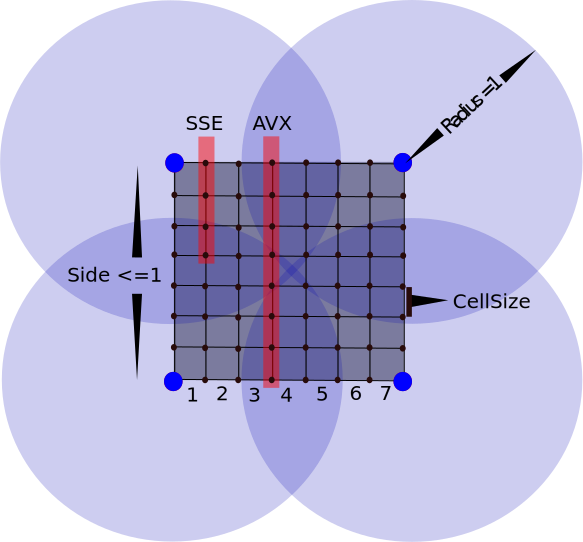
\includegraphics[width=0.9\linewidth]{figures/cpupoly/MPU.pdf}
  \caption{\label{fig:MPU}
  {The \textit{MPU} is our unit of computation per each core illustrated as a 2D cross section here. 
  Field-values due to every 4 or 8 points are computed in parallel with SSE or AVX instructions, respectively. 
  When the field at a vertex is zero no iso-surface will pass in the neighborhood of a unit circle (sphere in 3D) centered at that vertex.}
}
\end{figure}


\section{Algorithm}\label{sec:algorithm}
The input to our algorithm is a \blob data structure, representing an implicit model whose iso-surface we wish to find. Output is a 
triangle mesh.  The model bounding box and the cellsize parameter supplied by the user to control the resolution of the final mesh.
The \blob structure is first converted into a compact, linear structure required for SIMD optimization techniques, then the model 
bounding box is divided into the \textit{MPUSET} with respect to the \textit{cellsize} parameter.
The \textit{MPUSET} is processed in parallel using multiple cores; with a fast empty \textit{MPU} rejection method and SIMD surface 
extraction algorithm the mesh contained within intersecting $MPU$s is extracted. The algorithm has no synchronization points except after 
all \textit{MPU}s are processed and the triangle mesh is sent to the GPU for rasterization. The left column in figure 
(\ref{fig:AlgorithmHighLevelView}) displays these preparation steps in order.
The following sections describe this whole process in detail.


We start by describing the initialization phase and continue with the surface extraction details in the next section.
The algorithm starts by computing the size of an \textit{MPU} side (7 cells) and dividing the bounding box of the model into a 
3D grid of \textit{MPU}s, where each \textit{MPU} is assigned a unique global identifier. The main idea of our algorithm is parallel 
processing of the set of all \textit{MPU}s (\textit{MPUSET}) using multicore and SIMD processing techniques.

Our algorithm recursively splits \textit{MPUSET} into disjoint \textit{MPURANGE}s where each \textit{MPURANGE} is assigned to an idle core on 
the processor. The granularity of the divisions can be determined by the average amount of machine cycles spent to process an \textit{MPU}, 
however, in our implementation we resort to the solution provided by Intel Threading Building Blocks (TBB) \cite{Reinders2007}, 
which provides a non-preemptive task scheduling system to take care of the differences in task loads by 
monitoring processors and starting new tasks on idle cores automatically (work-stealing) \cite{Reinders2007}.


\begin{figure}[H]
  \centering
  % the following command controls the width of the embedded PS file
  % (relative to the width of the current column)
  \includegraphics[width=0.9\linewidth]{figures/cpupoly/AlgorithmHighLevelView}
  \caption{\label{fig:AlgorithmHighLevelView}
  {Left Column: The one-time preparation steps before scheduling kernel functions for computation.
  Middle Column: The early discard kernel function. Right Column: The $MPU$ processing kernel function.}
}
\end{figure}

\subsection{BlobTree Linearization}\label{sec:linearization}
The first step in our algorithm is the \blob reduction and pruning as suggested by Fox \etal \cite{Fox2001}.
In the second step, using the same linearization algorithm proposed for quadtrees \cite{Lee2000}; the \blob is converted into 
a pointerless representation to achieve cache-memory efficiency by keeping all input data structures at 
aligned memory addresses and fitting the entire \blob model into the last level cache memory of the processor. 
The final linearized \blob is in the format cache-line aligned structure of arrays. With this format several computations
can be optimized with SIMD instructions, e.g. applying a transformation matrix on a vector of 4 or 8 vertices as opposed to
scalar computation. The output mesh is also in the format of cache-line aligned structure of arrays which is the key to
compute colors and normals in SIMD fashion. 



\subsection{Surface Extraction}\label{sec:surfaceextraction}
In our algorithm we assign field values for every vertex of every \textit{MPU} that is not trivially rejected with the method explained in 
the following, and compute the triangular mesh representing the iso-surface. This approach combines elements of several algorithms 
(\cite{Wyvill1986, Lorensen1987, Bloomenthal1994a}).

We extended the method proposed by Zhang \etal \cite{Zhang2006} to trivially reject all empty \textit{MPU}s.
The observation made is that according to equation \ref{eq:WyvillFunc}, if the field value at a given vertex is zero then 
the shortest distance from that vertex to the iso-surface is greater than or equal to one (See figure \ref{fig:MPU}). Using 
this fact empty \textit{MPU}s can be identified very fast by evaluating the fields at the 8 vertices of each \textit{MPU} and rejecting it of all 8 
fields are zero. However, this test is only applicable when the cellsize parameter is smaller than or equal to $1/7$ or 0.1428. 
For larger \textit{cellsize}s the iso-surface may still intersect with the \textit{MPU} while the fields at vertices of the \textit{MPU} are zero. 
This process is depicted in the middle column of figure (\ref{fig:AlgorithmHighLevelView}).
For a discussion on \textit{cellsize} versus performance see section~\ref{sec:results}.

For larger \textit{cellsize}s we shoot 8 rays from the center of the \textit{MPU} to its eight vertices, using  the technique of Zhang \etal per 
each step we march $0.866c$ (0.866 is half of the diagonal of an \textit{MPU} with side one and $c$ being the cellsize parameter) along each ray. 
At each step we compute the fields for the 8 vertices along the rays; if a non-zero field is found then the \textit{MPU} is further processed, 
otherwise we march along the rays until we reach the vertices of the \textit{MPU}. 

If an \textit{MPU} is not rejected then it is further processed for surface extraction. A local copy of the linearized \blob is provided 
per each core in order to avoid \textit{false-sharing} among cores \cite{Bolosky1993}. Using SIMD processing techniques field values for all
512 vertices of \textit{MPU} are computed. With SSE or AVX instructions this step requires 128 or 64 field evaluation kernel runs, 
respectively (figure \ref{fig:MPU}).

All the fields are stored in a memory aligned array of 512 floating points. This technique avoids reevaluating field values while processing
cells in the next step. Storing field values from a SIMD register into memory aligned address can be accomplished with a SIMD instruction in
parallel. After this step all 343 cells of the \textit{MPU} are processed. Per each cell, the 8 vertex field values 
are gathered in SIMD fashion. Each vertex with a field greater than or equal to \textit{iso-value} is labeled one otherwise zero. 
The configuration index of the cell is computed using the SIMD method shown in algorithm \ref{alg:cellconfig}. A configuration index 
is computed to access the table as in \cite{Lorensen1987}. We used the modified marching cubes table proposed by Dietrich \etal that eliminates many 
of the degenerate triangles produced in the original MC algorithm \cite{Dietrich2009}. For the ambiguous cases we take another sample 
from the center of the cell \cite{Wyvill1986, Dietrich2009}. 

%bw - make this English
\begin{algorithm}[H]
\caption{SIMD computation of cell configuration. Pseudo code provided for AVX SIMD computation. Similar code can be written in SSE.}
\label{alg:cellconfig}
\begin{algorithmic}[1]	
  \STATE Gather the 8 vertex field values of the cell  
  \STATE simd $index = cmp\_ge8(fields, simd(0.5))$
  \STATE $index = and8(index, simd(1.0))$
  \STATE $index = mul8(index, maskPower)$  
  \STATE $index = hadd8(index, index)$   
\end{algorithmic}
\end{algorithm}

In algorithm (\ref{alg:cellconfig}) fields is an array of 8 vertex field values, 
line 2 performs a parallel comparison between \textit{iso-value} and fields. 
In line 4 maskpower shifts the field values into the appropriate slot in the SIMD array and finally line 5
performs a horizontal add operation on the values to compute the configuration index.

For each intersecting edge there is one inside and one outside vertex.
Using a root finding method the point of intersection of the iso-surface is computed and stored in a 
hash table to be reused by the neighboring cells that share that vertex. 

For the root finding methods that do not require gradient information such as regula falsi or bisection method, 
the field value should be evaluated multiple times along the edge, which will degrade the performance of the system. Other methods 
such as Newthon-Raphson require gradient information, and as mentioned in equation (\ref{eq:Normal})
each gradient computation involves 4 extra field evaluations. We describe a root finding
%%%  is this really new???/ 
technique based on SIMD instructions that computes the root with only one extra field evaluation in AVX (two with SSE) 
with adequate precision. By subdividing the intersecting edge into 8 vertices and evaluating the field values, the exact interval 
containing the final root can be identified. Performing linear interpolation in that interval will produce the 
final root (figure \ref{fig:root}), it is trivial to show when the number of intervals increases the interpolation error decreases \cite{Matthews1987}. 

\begin{figure}[H]
  \centering
  % the following command controls the width of the embedded PS file
  % (relative to the width of the current column)
  \includegraphics[width=0.8\linewidth]{figures/cpupoly/root.pdf}
  \caption{\label{fig:root}
  {Top: A cell edge is intersected with part of the surface shown in blue.  By performing one field evaluation using 
  AVX or two with SSE instructions the interval containing the intersection point can be identified. 
  The final root is computed using linear interpolation within the interval marked with bold line segment.}
}
\end{figure}


Algorithm (\ref{alg:surfaceextraction}) summarizes the process of surface extraction which is run per each \textit{MPU}. 
Lines 1 through 25 are related to the \textit{MPU} discard method explained earlier in this section. Lines 26 through 42
shows the cell processing technique which is optimized using SIMD cell configuration computation and our root 
finding method. Since color and normal attributes should only be computed for final mesh vertices, this step is 
performed last to fully leverage SIMD optimizations by performing every 4 or 8 attribute computations in 
one SIMD call which greatly enhances the throughput of the system and minimizes \blob traversals.

%%bw check this for undefined stuff - make ENglish
\begin{algorithm}
\caption{Algorithm for surface extraction of an \textit{MPU} using AVX SIMD instructions,
Similar code can be written for SSE instruction set. 
Input is linearized \blob $T$, lower vertex of \textit{MPU} and the \textit{cellsize} parameter. 
Output is the local mesh contained in the \textit{MPU}}
\label{alg:surfaceextraction}
\begin{algorithmic}[1]		
	\STATE $side \gets cellsize*7$
	\STATE simd $v \gets $Compute \textit{MPU} vertices
	\IF{$side \leq 1$}	
	\STATE simd $f \gets T.compute\_field8(v)$
	  \IF{$f == 0$}
	  \STATE return;
	  \ENDIF	
	\ELSE 
	  \STATE $flag \gets true$
	  \STATE $incr = 0.866*cellsize$	  
	  \STATE $d = incr$
	  \WHILE{$d \leq side * 0.866$}	
	  \STATE Shoot rays from center of \textit{MPU} to its 8 vertices
	  \STATE simd $v \gets $Travel along the rays for distance $d$     
	  \STATE simd $f \gets T.compute\_field8(v)$
	  \IF{$f != 0$}
	  \STATE $flag \gets false$
	  \STATE $break$;
	  \ENDIF
	  \STATE d = d + incr;
	  \ENDWHILE	
	  \IF{$flag == true$}
	  \STATE return;
	  \ENDIF	
	\ENDIF	
	
	\STATE float fieldCache[512];
	\FORALL{simd $vertex$ in $mpu$ vertices}
	\STATE simd $f \gets T.compute\_field8(vertex)$
	\STATE Store $f$ in appropriate location in $fieldCache$
	\ENDFOR
	
	
	\FORALL{$cell$ in $mpu$}
		\STATE $f \gets gather8(cell, fieldCache)$
		\STATE $edges \gets $Compute cell config from $f$ to access table
		\FOR{$i=1 \to $count of edges}
			\IF{root for $i$th edge is not stored in edge table}
			\STATE Compute and store root associated with $i$th edge		
			\STATE Add root to mesh vertices
			\ENDIF
		\ENDFOR				
		\STATE Add $cell$ triangles to mesh
	\ENDFOR	
	
	\STATE compute color and normal for all vertices (every 8 vertices in parallel)
\end{algorithmic}
\end{algorithm}


\section{Results}\label{sec:results}
We have implemented our algorithm using Intel threading building blocks in C++ on a Linux platform. We used two systems with 
different configurations. On the first system which has Intel i7-3960X processor with Sandy Bridge architecture, there are 6 
physical cores given that each core runs in hyper-threaded mode; up to 12 threads can run in parallel on this machine. 
This processor supports both SSE and AVX instructions and there is a last level cache memory of 15 megabytes 
which is shared between all cores.

The second system is a server with 4 Intel X7560 processor with Nehalem architecture. Each processor has 8 physical cores
or 16 in hyper-threaded mode and has 24 megabytes of last level cache memory and it does not support AVX instructions. 
Together these 4 processors provide us with as many as 32 physical cores (64 when hyper-threaded) on this server. 
We refer to these two systems with SNB and NHM respectively.


On the first experiment our goal was to prove the scalability of our algorithm. Figures (\ref{fig:PerfSNBTower}, \ref{fig:PerfXeonTower}) 
show the average running time of the algorithm when rendering towers model (figure \ref{fig:ModelTower}) on SNB and NHM systems, 
respectively. The \blob of the towers model has 7360 operators and 7296 primitives and a depth of 64 levels. 
In this test the cellsize parameter kept as a constant value of 0.14 which we found it to be a balance between number of triangles produced and 
the quality of the output mesh.  

In order to show the effect of SIMD optimizations we have tested our algorithm with scalar, 4-wide SSE and 8-wide AVX instructions. 
SSE being on average 4.58x faster than scalar and AVX being on average 7.35x faster than scalar run. As illustrated in figure \ref{fig:PerfSNBTower}
when the number of threads increases past 6, two threads run on every core; sharing hardware resources on the hyperthreaded cores.  
The slope is reduced because each thread gets less resources than it would if it ran alone on the core.  Past 12 threads, we 
schedule multiple threads per core, and they start to thrash the cache; making the algorithm memory bound.

Figure \ref{fig:PerfXeonTower} shows the performance of our algorithm when running on the NHM system. Doubling number of 
threads, doubled the performance of the algorithm on this machine up to 33rd thread. The same behavior is shown and hyper-threaded 
cores start to compete for memory access when having more than 32 threads running on this machine.

\begin{figure}[H]
  \centering
  \includegraphics[width = 1.0\linewidth]{figures/cpupoly/Perf_SNB.pdf}
  \caption{\label{fig:PerfSNBTower}
  {Average polygonization time of the towers model when running on SNB processor. Horizontal axis is the number of threads. 
  Vertical axis is time measured in milliseconds.}
}
\end{figure}

\begin{figure}[htb]
  \centering
  \includegraphics[width = 1.0\linewidth]{figures/cpupoly/Perf_NHM.pdf}
  \caption{\label{fig:PerfXeonTower}
  {Average polygonization time of the towers model when running on NHM processor. Horizontal axis is the number of threads. 
  Vertical axis is time measured in milliseconds.}
}
\end{figure}

%\begin{center}
\begin{table}[H]
\begin{center}
\caption{\label{table:speedup}{Comparison of speedups and field value evaluations per triangle (\textit{FVEPT}) for polygonization of Tower model 
  with different SIMD instruction sets. Note that FVEPT was 17 before adding SIMD optimizations.}}
  \begin{tabular}{ | l | c | c | c | }
    \hline    
    Processor & SIMD Method & Speedup & FVEPT \\ \hline \hline    
    SNB & SSE & 4.58x & 4 \\ \hline
    SNB & AVX & 7.35x	& 2 \\ \hline
    NHM & SSE & 4.25x & 4 \\    
    \hline
  \end{tabular}
  	
\end{center}
\end{table}
%\end{center}

Table \ref{table:speedup} shows the effect of using SIMD optimizations in our algorithm. With SSE and AVX the theoretical speedups are 4 and 8 times, 
respectively. Due to memory alignment techniques and proper caching mechanisms the speedup with 4-wide SSE is greater than 4. The AVX speedup can be 
improved more once scatter/gather instructions are implemented on the SNB processors which will improve the performance of surface extraction algorithm.
Number of field evaluations per triangle shows the average amount of times the field evaluation kernel called to compute a single vertex in the output mesh. 

In another experiment we studied the effect of our early discard method when the side of each \textit{MPU} is less than one 
(figure \ref{fig:DiscardEffect}). Starting from a large cellsize, we reduced the cellsize in uniform steps and measured the polygonization time. 
The red curve shows the polygonization time when the discard method described in section \ref{sec:surfaceextraction} is not being used and the blue curve 
is the timing when that method is in effect. Note that with the blue curve as soon as the \textit{MPU} side is less than one; (\textit{cellsize} = 0.14) empty 
\textit{MPU}s started to get discarded efficiently thus the constant part of the time value is reduced at that point.

\begin{figure}[htb]
  \centering
  \includegraphics[width = 1.0\linewidth]{figures/cpupoly/DiscardEffect2.pdf}
  \caption{\label{fig:DiscardEffect}
  {Reducing cellsize parameter results in more \textit{MPU} generation and increase in polygonization time.
  However, at a certain cellsize our early discard method stops polygonization time increase by rejecting 
  all empty \textit{MPU}s more efficiently.}
}
\end{figure}



%\ref{fig:ResultScaleSNBTower}, \ref{fig:ResultScaleXeonTower}
Figure \ref{fig:TowerSNBTimeBreakDown} shows the polygonization time breakdown when rendering the towers model on SNB processor. 
Horizontal axis is the core number for a total of 12 cores on that system. As can be seen from the top of this chart; 
the idle time is very short and the cores are active almost all the time. This shows that the work stealing algorithm scales well. 
190463 \textit{MPU}s are processed and 116723 of them are intersected with the iso-surface (40 percent were empty).
40 percent of the \textit{MPUSET} has been processed in less than 10 percent of the total polygonization time.

\begin{figure}[htb]
  \centering
  \includegraphics[width = 1.0\linewidth]{figures/cpupoly/PerCoreTimeBreakDown.pdf}
  \caption{\label{fig:TowerSNBTimeBreakDown}
  {Towers model per-core time breakdowns. Each bar represents a logical core on the processor for a total of 12 cores. 
  Vertical axis is the total polygonization time. 190463 \textit{MPU}s processed with 12 cores in 9283 milliseconds. 
  This chart shows the portion of time spent in each step of the algorithm when rendering the towers model on the 
  SNB processor with 8-wide AVX instructions.}
}
\end{figure}

\begin{figure}[htb]
  \centering
  % the following command controls the width of the embedded PS file
  % (relative to the width of the current column)
  \includegraphics[height = 0.8\linewidth]{figures/cpupoly/towers64}
  \caption{\label{fig:ModelTower}
  {Towers model created with skeletal primitives and binary operators in 
  our incremental designing system. The model is a grid of 8 by 8 towers for a total of
  7360 operators and 7296 primitives.}
}
\end{figure}

\begin{figure}[htb]
  \centering
  % the following command controls the width of the embedded PS file
  % (relative to the width of the current column)
  \includegraphics[width=0.7\linewidth]{figures/cpupoly/medusa}
  \caption{\label{fig:ModelMedusa}
  {Medusa model courtesy of Schmidt \etal \cite{SWG2005}.}
}
\end{figure}

These results demonstrate the scalability of our algorithm both in the number of SIMD vector lines and 
the number of cores available on each processor. 

Finally, we compare our method against Schmidt \etal's \cite{SWG2005} using the Medusa model provided by them   
which has 2920 primitives and 11 operators and the tree structure has a depth of 6 (figure \ref{fig:ModelMedusa}).
In this experiment, we divided polygonization timings reported in \cite{SWG2005} by 8 as the best AVX
optimized version of Schmidt's method. Then we ran our polygonization algorithm
optimized with AVX instructions on a single core for Medusa model (See table \ref{table:stats}). 

\begin{table}[H]
\begin{center}
	 \caption{\label{table:stats}
  {Comparison of our polygonization method against Schmidt \etal's \cite{SWG2005} 
  when rendering Medusa model at 5 different resolutions on one single core with AVX instructions. 
  All timings are in milliseconds.}
}
  \begin{tabular}{ | c | c | c | c |}
    \hline    
    CellSize & Our method & Schmidt's method & Speedup \\ \hline \hline
    0.01 & 5220 & 6228 & 1.19x\\ \hline
    0.03 & 3441 & 3653 & 1.06x \\ \hline
    0.05 & 1071 & 2175 & 2.03x	 \\ \hline
    0.10 & 264 & 1292 &	4.89x \\ \hline    
    0.14 & 108 & 721 & 6.67x \\        
    \hline
  	\end{tabular}
\end{center}
\end{table}


The results shows that our algorithm outperforms that of Schmidt \etal by a factor of 6 when running on a single core in lower resolutions. 

\section{Chapter Conclusions}\label{sec:futurework}
In this chapter we presented a new parallel polygonization algorithm using SIMD processing techniques that takes advantage of 
a multi-core machine. Our main contribution is a scalable algorithm both in terms of the number of cores available on 
multicore architectures and the number of SIMD vector width as shown in the results section.  We also presented a SIMD technique for 
finding the intersection of an iso-surface and a cube edge.

%\section{Acknowledgement}
%We would like to thank Intel Corporation for their support and providing us with their cutting-edge server and processors.
%This work is partly supported by the GRAND NCE foundation of Canada, and the Natural Sciences and Engineering Research Council of Canada.
